\chapter{Fundamentação Teórica}
\label{cap:fundamentacao-teorica}

\section{Engenharia de Software}
\label{sec:engenharia-de-software}

Sommerville (2007) definiu engenharia de software como uma disciplina da engenharia que cuida de todos os aspectos da produção de software, desde a especificação do sistema até a sua manutenção, depois que ele entra em operação.\\ 
A engenharia é constituída de processos de software, que são conjuntos de atividades e resultados para se produzir um software. Existem quatro atividades fundamentais, são elas: 
Especificação de Software: o software a ser desenvolvido e as restrições para sua operação são definidos. 
Desenvolvimento de Software: o software deve ser feito atendendo suas especificações.\\ 
Validação de Software: o software tem de ser validado para garantir que está em cima do que o cliente deseja. 
Evolução do Software: o software sofre modificações para atender as necessidades do cliente. 
No desenvolvimento de software, o principal objetivo é a criação de sistemas que atendam às necessidades dos clientes e usuários, ou seja, uma correta especificação dos requisitos se torna essencial para que o desenvolvimento tenha sucesso. Uma forma de entender melhor esses requisitos é dividindo-os em: Requisitos Funcionais e Requisitos Não-Funcionais, Vasconcelos, Rouiller, Machado e Medeiros (2006).\\
Os Requisitos Funcionais definem as funções que componentes do sistema ou sistemas devem executar. 
Os Requisitos Não-Funcionais incluem limitações no produto, como por exemplo: desempenho, confiabilidade, segurança e limitações no desenvolvimento, como custos e tempo, componentes a serem reutilizados, entre outros.

\section{Desenvolvimento Mobile}
\label{sec:desenvolvimento-mobile}

Um dispositivo móvel pode ser definido como um computador de bolso, normalmente composto de uma tela e um teclado em miniatura podendo estes serem combinados em um so dispositivo conhecido como \textit{ touchscreen}.

Características dos dispositivos moveis:

\begin{alineascomponto}
 
\item Pequeno em tamanho
\item Baixo consumo de energia
\item Curto tempo de inicialização
\item Armazenamento de dados local e/ou remoto

	\end{alineascomponto}


Os dispositivos moveis mais populares são:

\begin{alineascomponto}
 
\item Smartphones
\item Tablets
\item Console portátil
\item Notebooks

	\end{alineascomponto}


Toda esta tecnologia que possibilita a existência dos dispositivos moveis começou a partir do primeiro celular inventado, em 3 de abril de 1983, o Motorola DynaTAC 8000x. Foi então que em 1992 a empresa Apple lançou no mercado o primeiro PDA que continha memoria de 1MB e tela sensível ao toque, desde então esta tecnologia tem se desenvolvido e mostrado como
vantagem  a possibilidade dos dados serem acessados em qualquer lugar a qualquer hora.

Dentre os dispositivos moveis citados, o que mais se destacam são os smartphones.
Um smartphone (telefone inteligente) poder ser definido como um celular que possui muitas funções. Essas funções são realizadas de maneira mais eficientes do que um celular normal, em geral possuem internet wiFi, navegadores, é possível realizar a instalação de aplicativos e possui um Sistema Operacional (SO). 

Uma das grandes vantagens dos smartphones é a capacidade de qualquer pessoa desenvolver um aplicativo para o aparelho pois, em geral, o SO é um software aberto, onde existe a flexibilidade da criação de aplicativos.

Um Sistema Operacional é um conjunto de programas responsável por alocar recursos do hardware fornecendo também uma interface para o usuário. Os sistemas operacionais para smartphones mais conhecidos atualmente são:iOS, Android, Windows Mobile e BlackBerry

Segundo uma pesquisa realizada pela Gartner, o sistema operacional mais vendido em 2015 (para smartphones) foi o Android e em segundo o iOS, conforme pode ser visto na imagem abaixo.
\begin{figure}[h!]
		\centering
		\Caption{\label{fig:exemplo-1}Venda Mundial de Smartphones por Sistemas Operacionais}	
		\UECEfig{}{
			\fbox{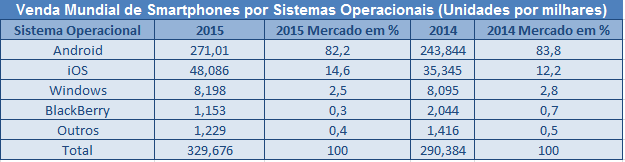
\includegraphics[width=12cm]{figuras/GartnetSamart}}
		}{
			\Fonte{Gartner (Agosto 2015)}			
		}	
	\end{figure}

\subsection{Aplicativos Moveis}


Estes aplicativos desenvolvidos para dispositivos moveis podem ser nativos, web e híbridos. Em uma pesquisa realizada pela Gartner em 2013 constata que entre as 10 maiores necessidades para o mercado, no quesito aplicativo esta os jogos e entretenimento moveis, reporta também que este mercado esta em constante crescimento.
\begin{comment}
http://www.telefonescelulares.com.br/o-que-e-smartphone/
http://pt.slideshare.net/cetorres/palestra-mobilidade-computao-mvel-dispositivos-e-aplicativos-2013
\end{comment}

\subsection{Android}

\section{Scrum}
\label{sec:scrum}

Scrum é uma metodologia ágil para gestão e planejamento de projetos de softwares e sua base fundamental pode ser bem descrita na imagem abaixo.

	\begin{figure}[h!]
		\centering
		\Caption{\label{fig:exemplo-2}Prática do Scrum}	
		\UECEfig{}{
			\fbox{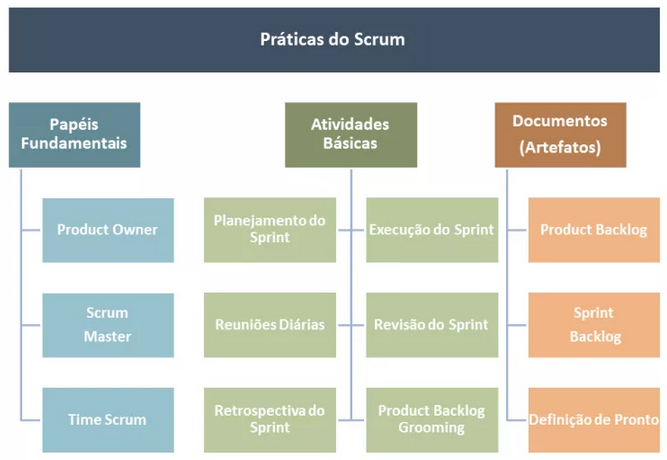
\includegraphics[width=13cm]{figuras/PraticaScrum}}
		}{
			\Fonte{Elaborado pelo autor}			
		}	
	\end{figure}

Cada equipe de Scrum, geralmente, possuem 3 papeis:
\begin{alineascomponto}
	\item ProductOwner
É responsável por decidir os recursos e funcionalidades utilizadas no projeto é também sua responsabilidade manter clareza no objetivo do projeto, para que haja uma melhor interação o ProductOwner geralmente colabora com o ScrumMaster.

	\item ScrumMaster
É de sua responsabilidade ajudar todos envolvidos a entender os valores, princípios e práticas do Scrum. Também fica responsável por melhorias no uso do Scrum e está sempre orientando para que não haja a perda de foco. 

	\item Development Team
São todos da equipe responsáveis pelo desenvolvimento em si do software, possuem papeis como: arquiteto, testador, programador e etc.. Para esta equipe é recomendável que se organizem para determinar a melhor maneira de realizar o trabalho.

	\end{alineascomponto}
	
	
	A imagem abaixo representa o processo de interação das atividades

	\begin{figure}[h!]
		\centering
		\Caption{\label{fig:exemplo-3} Interação das atividades }	
		\UECEfig{}{
			\fbox{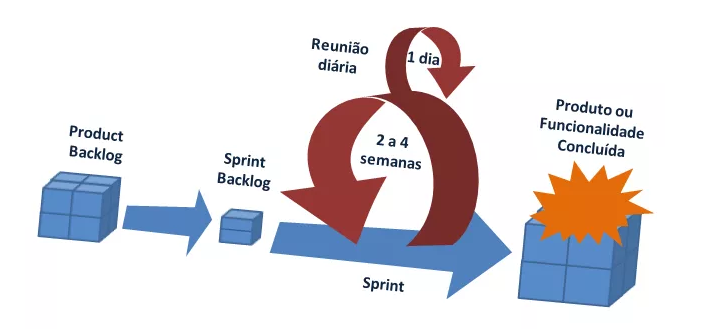
\includegraphics[width=13cm]{figuras/InteracaoScrum}}
		}{
		\Fonte{Elaborado pelo autor}			
	}	
	\end{figure}
	O ProductOwner tem a visão final do produto, representado na figura como grande cubo. Este cubo é "divido" em vários outros cubos pequenos, este chamado de ProductBacklog.\\
O ProductBacklog pode ser descrito, em uma forma simplificada, como pequenas etapas/objetivos para se chegar ao produto final.
Para planejar a prioridade dos Backloge também quando e quanto tempo durará seu desenvolvimento, é utilizado o Sprint.\\
O Sprint tem duração mediana de 2 a 4 semanas, mas é também flexível dependendo do tempo desenvolvimento final estimado no começo do planejamento.\\

Também existe a técnica do Daily Scrum, utilizado para o desenvolvimento deste jogo junto a sua monografia. Para o Daily Scrum, é utilizado as três perguntas consideradas básicas para haver um melhor desenvolvimento de todos da equipe.\\
Estas são:\\ 
\textbf{1}- O que fiz ontem que ajudou o time a atingir a meta do Sprint?\\
\textbf{2}- O que vou fazer hoje para ajudar o time a atingir a meta do Sprint?\\
\textbf{3} - Existe algum impedimento que não permita a mim ou ao time atingir a meta do Sprint?\\
Para a utilização do método Scrum há várias outras técnicas existentes, porém devido ao tempo curto e a quantidade de integrantes dispostos no desenvolvimento do jogo Caapora, foi somente utilizado os métodos acima.


\section{Controle de Versão}
\label{sec:Controle-de-Versão}

O controle de versão tem como objetivo a gerencia de versões de um mesmo projeto. Vários programadores podem trabalhar em um mesmo projeto sendo possível manter um histórico de atualizações.
Dentre as infinidades de vantagens para se utilizar um "controlador de versões" as três principais que se destacam são:
\begin{alineascomponto}
	
   \item Possibilidade de salvar o histórico
   \item Possibilidade de desenvolver versões diferentes
   \item Possibilidade de se programar em paralelo

	\end{alineascomponto}

\subsection{Funcionamento}\\
Os históricos contendo as modificações de cada versão ficam armazenados em um repositório (servidor). Este processo dá à liberdade para que o desenvolvedor possa baixar a última versão, trabalhar em seu código e posteriormente atualizar a versão já previamente armazenada no servidor.
	\begin{figure}[h!]
		\centering
		\Caption{\label{fig:exemplo-4} Ut posuere, ex quis sagittis auctor, magna massa euismod felis}	
		\UECEfig{}{
			\fbox{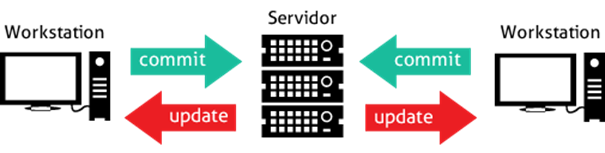
\includegraphics[width=13cm]{figuras/ControleVersao}}
		}{
		\Fonte{Elaborado pelo autor}			
	}	
	\end{figure}
	
	Para que seja realizada a sincronização entre a 'workstation' e o servidor é necessário utilizar os comandos:
	
	\begin{alineascomponto}
\item Commit - realiza o envio das alterações realizadas para o servidor gerando um novo histórico de atualizações.
\item Update - realiza o envio da última versão contida no servidor para a workstation.

	\end{alineascomponto}

\section{Inteligência Artificial}
\label{sec:inteligencia-artificial}

A Inteligência Artificial (IA) é um ramo de pesquisa da ciência da computação que procura através de meio computacionais desenvolver mecanismos e/ou dispositivos que simulem a capacidade do ser humano de raciocinar e resolver problemas, ou seja, ser inteligente. 

O campo de IA tem como objetivo, o contínuo aumento da "inteligência" do computador, pesquisando, para isto, também os fenômenos da inteligência natural. Para este fim, IA é definida  como sendo uma coleção de técnicas suportadas por computador emulando algumas capacidades dos seres humanos. Esta coleção inclui:

\begin{alineascomponto}
	
   \item Resolução de problemas
   \item Compreensão de Linguagem Natural
   \item Visão e Robótica
   \item Sistemas Especialistas e Aquisição de Conhecimento
   \item Metodologias de Representação de Conhecimento

	\end{alineascomponto}
	
	Hoje em dia a Inteligência Artificial é utilizada em vários fins, não só exclusivamente para informática e um dos pontos em que se destaca é para o desenvolvimento de jogos. Primeiramente utilizada em jogos clássicos como xadrez ou jogo da velha e atualmente utilizada para jogos digitais.
   Os algoritmos de IA desenvolvidos para jogos digitais podem ser divididos em três blocos:

\begin{alineascomponto}
	
   \item Movimento:\\
   De como um personagem é movimentado, do local de inicial ate o destino final, também determina o calculo do percurso, detectando objetos e desviando de obstáculos.
   
 \item Tomada de Decisão:\\
Cada personagem possui um conjunto de atividades e estados possíveis, estes sendo: estar parado, fugir, atacar adversário entre outros. Para que cada ação seja possível, a personagem precisara fazer uma tomada de decisão analisando o contexto. Esta decisão pode ser de ativar um algoritmo de movimento, alterar um estado interno ou a animação. Não necessariamente essas alterações serão visuais.

\item Estratégia:\\
A maioria dos jogos digitais desenvolvidos com IA ocorrem nos dois tipos já citados estes também podem conter personagens que trabalham em grupo ou equipe contando com uma tomada de decisão individual.

	\end{alineascomponto}

	
As pesquisas iniciaram-se na Segunda Guerra Mundial com os cientistas Hebert Simon, Allen Newell,  Jonh McCarthy com o objetivo em comum de reproduzir uma maquina que simulasse o cérebro humano. (SANTOS,2015) 
	
	
	
	
	
